\documentclass[conference]{IEEEtran}
\usepackage{cite}
\usepackage{amsmath,amssymb}
\usepackage{graphicx}
\usepackage{booktabs}
\usepackage{xcolor}
\usepackage{url}
\usepackage[hidelinks]{hyperref}

% Every number in the text comes from these generated files (see reproduce.sh).
% Generated by analyze.py. Do not edit by hand.
\providecommand{\err}[2]{\ifcsname err-#1-#2\endcsname\csname err-#1-#2\endcsname\else\textcolor{red}{[#1-#2 missing]}\fi}
\providecommand{\errmean}[2]{\ifcsname errmean-#1-#2\endcsname\csname errmean-#1-#2\endcsname\else\textcolor{red}{[#1-#2 missing]}\fi}
\providecommand{\errbest}[2]{\ifcsname errbest-#1-#2\endcsname\csname errbest-#1-#2\endcsname\else\textcolor{red}{[#1-#2 missing]}\fi}
\providecommand{\nruns}[2]{\ifcsname nruns-#1-#2\endcsname\csname nruns-#1-#2\endcsname\else\textcolor{red}{[#1-#2 missing]}\fi}
\expandafter\def\csname err-plain-20\endcsname{9.56 $\pm$ 0.20}
\expandafter\def\csname errmean-plain-20\endcsname{9.56}
\expandafter\def\csname errbest-plain-20\endcsname{9.39}
\expandafter\def\csname nruns-plain-20\endcsname{3}
\expandafter\def\csname err-plain-32\endcsname{9.89$^{\dagger}$}
\expandafter\def\csname errmean-plain-32\endcsname{9.89}
\expandafter\def\csname errbest-plain-32\endcsname{9.89}
\expandafter\def\csname nruns-plain-32\endcsname{1}
\expandafter\def\csname err-plain-44\endcsname{10.94$^{\dagger}$}
\expandafter\def\csname errmean-plain-44\endcsname{10.94}
\expandafter\def\csname errbest-plain-44\endcsname{10.94}
\expandafter\def\csname nruns-plain-44\endcsname{1}
\expandafter\def\csname err-plain-56\endcsname{12.79 $\pm$ 0.41}
\expandafter\def\csname errmean-plain-56\endcsname{12.79}
\expandafter\def\csname errbest-plain-56\endcsname{12.46}
\expandafter\def\csname nruns-plain-56\endcsname{3}
\expandafter\def\csname err-resnet-110\endcsname{6.50$^{\dagger}$}
\expandafter\def\csname errmean-resnet-110\endcsname{6.50}
\expandafter\def\csname errbest-resnet-110\endcsname{6.50}
\expandafter\def\csname nruns-resnet-110\endcsname{1}
\expandafter\def\csname err-resnet-20\endcsname{8.36 $\pm$ 0.27}
\expandafter\def\csname errmean-resnet-20\endcsname{8.36}
\expandafter\def\csname errbest-resnet-20\endcsname{8.09}
\expandafter\def\csname nruns-resnet-20\endcsname{3}
\expandafter\def\csname err-resnet-32\endcsname{7.78$^{\dagger}$}
\expandafter\def\csname errmean-resnet-32\endcsname{7.78}
\expandafter\def\csname errbest-resnet-32\endcsname{7.78}
\expandafter\def\csname nruns-resnet-32\endcsname{1}
\expandafter\def\csname err-resnet-44\endcsname{7.41 $\pm$ 0.30}
\expandafter\def\csname errmean-resnet-44\endcsname{7.41}
\expandafter\def\csname errbest-resnet-44\endcsname{7.06}
\expandafter\def\csname nruns-resnet-44\endcsname{3}
\expandafter\def\csname err-resnet-56\endcsname{7.93 $\pm$ 0.23}
\expandafter\def\csname errmean-resnet-56\endcsname{7.93}
\expandafter\def\csname errbest-resnet-56\endcsname{7.66}
\expandafter\def\csname nruns-resnet-56\endcsname{3}
\expandafter\def\csname err-resnet-56-fp32\endcsname{7.95$^{\dagger}$}
\expandafter\def\csname errmean-resnet-56-fp32\endcsname{7.95}
\expandafter\def\csname errbest-resnet-56-fp32\endcsname{7.95}
\expandafter\def\csname nruns-resnet-56-fp32\endcsname{1}
\expandafter\def\csname err-resnet-56-B\endcsname{7.06 $\pm$ 0.33}
\expandafter\def\csname errmean-resnet-56-B\endcsname{7.06}
\expandafter\def\csname errbest-resnet-56-B\endcsname{6.83}
\expandafter\def\csname nruns-resnet-56-B\endcsname{3}
\providecommand{\gap}[1]{\ifcsname gap-#1\endcsname\csname gap-#1\endcsname\else\textcolor{red}{[gap-#1 missing]}\fi}
\expandafter\def\csname gap-110\endcsname{0.07}
\expandafter\def\csname gap-20\endcsname{0.39}
\expandafter\def\csname gap-32\endcsname{0.27}
\expandafter\def\csname gap-44\endcsname{0.24}
\expandafter\def\csname gap-56\endcsname{0.96}
\providecommand{\trainerr}[2]{\ifcsname trainerr-#1-#2\endcsname\csname trainerr-#1-#2\endcsname\else\textcolor{red}{[train #1-#2 missing]}\fi}
\expandafter\def\csname trainerr-plain-20\endcsname{1.21}
\expandafter\def\csname trainerr-plain-32\endcsname{1.25}
\expandafter\def\csname trainerr-plain-44\endcsname{2.10}
\expandafter\def\csname trainerr-plain-56\endcsname{5.53}
\expandafter\def\csname trainerr-resnet-110\endcsname{0.02}
\expandafter\def\csname trainerr-resnet-20\endcsname{0.77}
\expandafter\def\csname trainerr-resnet-32\endcsname{0.32}
\expandafter\def\csname trainerr-resnet-44\endcsname{0.16}
\expandafter\def\csname trainerr-resnet-56\endcsname{0.15}
\providecommand{\cmpdiff}[1]{\ifcsname cmpdiff-#1\endcsname\csname cmpdiff-#1\endcsname\else\textcolor{red}{[#1 missing]}\fi}
\providecommand{\cmpt}[1]{\ifcsname cmpt-#1\endcsname\csname cmpt-#1\endcsname\else\textcolor{red}{[#1 missing]}\fi}
\expandafter\def\csname cmpdiff-A-vs-B-56\endcsname{0.86}
\expandafter\def\csname cmpt-A-vs-B-56\endcsname{3.7}
\expandafter\def\csname cmpdiff-56-vs-44\endcsname{0.52}
\expandafter\def\csname cmpt-56-vs-44\endcsname{2.4}
\expandafter\def\csname cmpdiff-plain56-vs-20\endcsname{3.23}
\expandafter\def\csname cmpt-plain56-vs-20\endcsname{12.2}
\providecommand{\totalruns}{23}

% Generated by layer_responses.py. Do not edit by hand.
\providecommand{\lstd}[2]{\ifcsname lstd-#1-#2\endcsname\csname lstd-#1-#2\endcsname\else\textcolor{red}{[#1-#2 missing]}\fi}
\expandafter\def\csname lstd-plain-20\endcsname{0.843}
\expandafter\def\csname lstd-plain-32\endcsname{0.727}
\expandafter\def\csname lstd-plain-44\endcsname{0.656}
\expandafter\def\csname lstd-plain-56\endcsname{0.608}
\expandafter\def\csname lstd-resnet-110\endcsname{0.336}
\expandafter\def\csname lstd-resnet-20\endcsname{0.752}
\expandafter\def\csname lstd-resnet-32\endcsname{0.626}
\expandafter\def\csname lstd-resnet-44\endcsname{0.520}
\expandafter\def\csname lstd-resnet-56\endcsname{0.455}

\graphicspath{{../results/}}

\newcommand{\repo}{\url{https://github.com/Royal93/resnet-repro}}

\begin{document}

\title{Does Depth Hurt Plain Networks and Help Residual Ones?\\
Reproducing the Degradation Claim of Deep Residual Learning on CIFAR-10}

\author{\IEEEauthorblockN{Royal Goronga}
\IEEEauthorblockA{School of Computer Science and Applied Mathematics\\
University of the Witwatersrand, Johannesburg, South Africa\\
Code and all run logs: \repo}}

\maketitle

\begin{abstract}
He \emph{et al.} \cite{he2016deep} claim that deeper plain networks suffer a \emph{degradation problem}, higher training and test error, while residual networks with parameter-free identity shortcuts improve with depth. I reimplemented their CIFAR-10 experiments (Section~4.2, Fig.~6, Table~6) in PyTorch and trained \totalruns{} models on a single laptop GPU. The qualitative claim reproduces clearly: plain-network test error rises from \err{plain}{20}\% at 20 layers to \err{plain}{56}\% at 56 layers (three seeds each), while ResNet error falls from \err{resnet}{20}\% at 20 layers to \errmean{resnet}{110}\% at 110 layers, within the paper's reported spread. The quantitative match is weaker in the middle: with the paper's zero-padding (option A) shortcuts, my ResNet-56 is \gap{56} points behind the paper's 6.97\% and is beaten by ResNet-44, consistently over three seeds. Full-precision training does not change this. Replacing only the three dimension-changing shortcuts with projections (option B) brings ResNet-56 to \err{resnet}{56-B}\%, matching the paper, which suggests the gap lies in an unstated detail of the zero-padding shortcut.
\end{abstract}

\begin{IEEEkeywords}
reproducibility, residual networks, degradation problem, CIFAR-10
\end{IEEEkeywords}

\section{The Claim}
\label{sec:claim}
The claim reproduced is the following, from Section~4.2 of \cite{he2016deep}:

\begin{quote}
\emph{On CIFAR-10, plain networks of 20, 32, 44 and 56 layers show higher training and test error as depth increases, whereas residual networks with identity (option A) shortcuts, and therefore exactly the same depth, width and parameter count, show lower error as depth increases, down to 6.43\% at 110 layers.}
\end{quote}

The evidence in the paper is Fig.~6 (training and test curves for plain networks on the left and ResNets in the middle) and Table~6 (ResNet test errors of 8.75, 7.51, 7.17, 6.97 and 6.43\% for 20, 32, 44, 56 and 110 layers). The authors support it with a controlled comparison: the networks are built from the same 6$n$+2 template with 16, 32 and 64 filters, and the residual versions differ \emph{only} by shortcuts that add no parameters. The plain networks' errors are shown only in Fig.~6, and only ResNet-110 is reported over several runs (best of five, mean $6.61\pm0.16$\%). Fig.~7 adds supporting analysis: residual layers have smaller response magnitudes than plain ones.

This claim was chosen because it is the paper's central argument, it can be tested at full scale on a 4\,GB laptop GPU, and it is falsifiable in both directions: degradation could fail to appear in plain networks, or shortcuts could fail to remove it.

\section{Route}
\label{sec:route}
I reimplemented the method from the paper's text in PyTorch \cite{paszke2019pytorch}. The authors' Caffe \cite{jia2014caffe} implementation was not used. The code (\repo) consists of a model definition (\texttt{models.py}), a training script following the paper's recipe (\texttt{train.py}), analysis scripts producing every table and figure in this report, and a single command, \texttt{reproduce.sh}, that runs everything.

The code was written with the help of an AI assistant. I chose the claim and the additional experiments in Section~\ref{sec:own}, ran every training run on my own laptop, checked the architecture, schedule and augmentation against the paper, dealt with problems during training, and interpreted the results.

\section{Setup}
\label{sec:setup}
\subsection{What matches the paper}
The architecture is the paper's: a 3$\times$3 convolution, then $3n$ residual blocks of two 3$\times$3 convolutions over feature maps of 32, 16 and 8 pixels with 16, 32 and 64 filters, global average pooling and a 10-way classifier, for 6$n$+2 weighted layers. Batch normalisation \cite{ioffe2015batch} follows each convolution, ReLU follows the shortcut addition, and weights use He initialisation \cite{he2015delving}. Shortcuts use option A: identity, with zero-padded extra channels and stride 2 where the size halves. My parameter counts (0.27M, 0.46M, 0.66M, 0.85M, 1.73M) match Table~6, and plain and residual networks have identical counts.

Training follows the paper exactly: SGD with momentum 0.9, weight decay 0.0001, batch size 128, learning rate 0.1 divided by 10 at 32k and 48k iterations, and stopping at 64k iterations. Augmentation is the 4-pixel padding, random 32$\times$32 crop and horizontal flip of \cite{lee2015dsn}, with per-pixel mean subtraction. Models train on all 50k training images and are tested on a single view of the 10k test images. ResNet-110 uses the paper's warm-up: learning rate 0.01 until training error falls below 80\%.

\subsection{What I changed}
Table~\ref{tab:diff} lists every known difference. The scale is \emph{not} reduced: the dataset, model sizes and schedule are the paper's. Only the hardware, framework and numerical precision differ.

\begin{table}[t]
\caption{Differences from the original setup}
\label{tab:diff}
\centering
\small
\begin{tabular}{@{}p{0.27\linewidth}p{0.3\linewidth}p{0.33\linewidth}@{}}
\toprule
Aspect & Paper & This reproduction \\
\midrule
Framework & Caffe & PyTorch \\
Hardware & 2 GPUs & 1 RTX 3050 laptop GPU (4\,GB) \\
Precision & FP32 & FP16 mixed precision \cite{micikevicius2018mixed}; one FP32 control run \\
Determinism & not stated & non-deterministic cuDNN kernels \\
Reported error & not stated (best of 5 for ResNet-110) & final error after 64k iterations \\
Runs per model & one value reported (5 runs for ResNet-110) & 3 seeds for depths 20, 44$^{*}$, 56; 1 for 32, 110 \\
Plain-net numbers & Fig.~6 only & tabulated \\
\bottomrule
\end{tabular}\\[2pt]
\raggedright\footnotesize $^{*}$Plain-44 has one seed.
\end{table}

\section{Results Next to the Paper's}
\label{sec:results}
Table~\ref{tab:main} compares final test errors like for like: same dataset, depths, parameter counts and schedule. Fig.~\ref{fig:depth} plots the same numbers against depth, and Fig.~\ref{fig:curves} shows the training curves in the style of the paper's Fig.~6.

\begin{table}[t]
\caption{CIFAR-10 test error (\%) by depth. Mean $\pm$ std over 3 seeds; $^{\dagger}$single run.}
\label{tab:main}
\centering
\small
\begin{tabular}{@{}rcccc@{}}
\toprule
Depth & Params & Plain (ours) & ResNet (ours) & ResNet (paper) \\
\midrule
20 & 0.27M & 9.56 $\pm$ 0.20 & 8.36 $\pm$ 0.27 & 8.75 \\
32 & 0.46M & 9.89$^{\dagger}$ & 7.78$^{\dagger}$ & 7.51 \\
44 & 0.66M & 10.94$^{\dagger}$ & 7.41 $\pm$ 0.30 & 7.17 \\
56 & 0.85M & 12.79 $\pm$ 0.41 & 7.93 $\pm$ 0.23 & 6.97 \\
110 & 1.73M & -- & 6.50$^{\dagger}$ & 6.43 \\
\bottomrule
\end{tabular}

\end{table}

\begin{figure}[t]
\centering
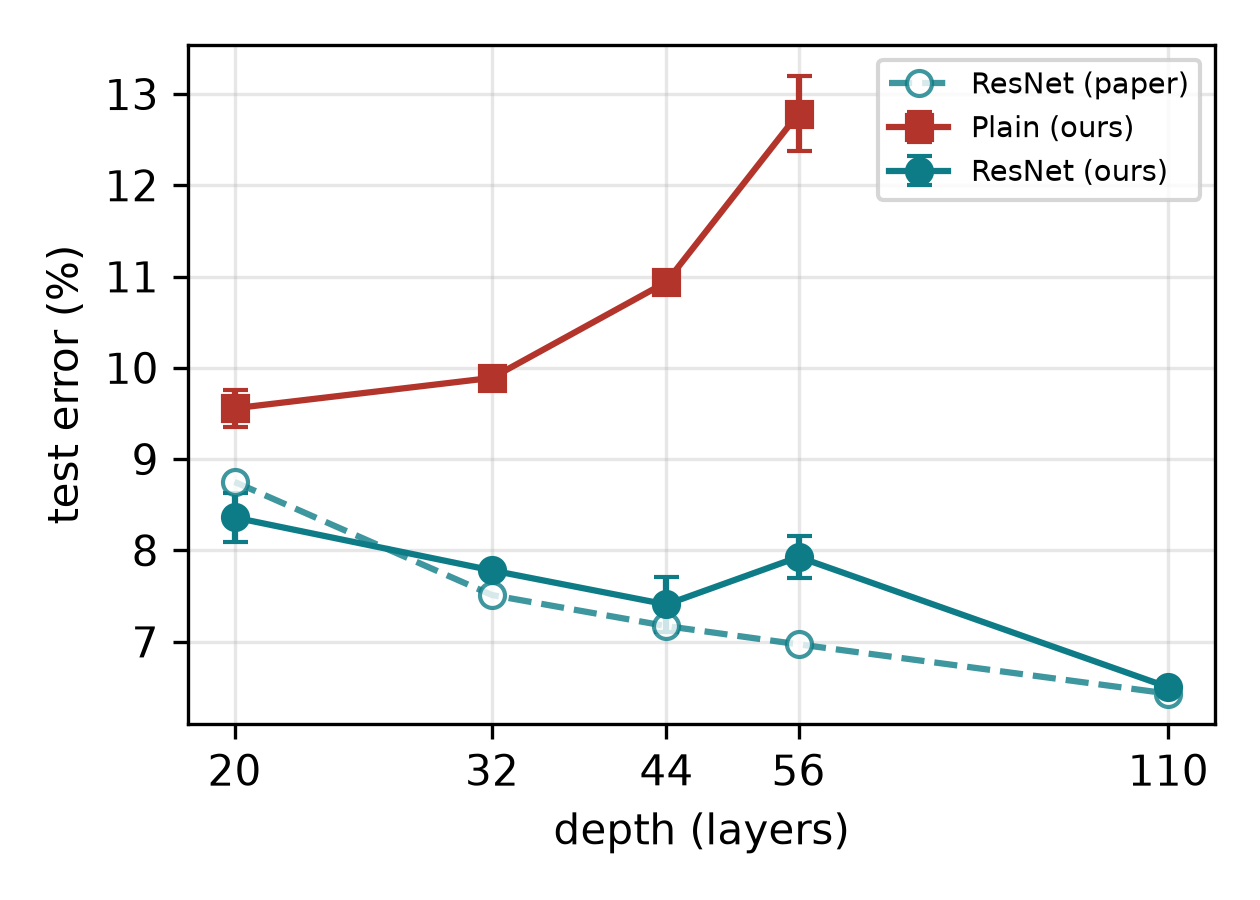
\includegraphics[width=\linewidth]{fig_depth.png}
\caption{Final test error against depth. Error bars are one standard deviation over three seeds. The paper's ResNet values (Table~6) are shown as open circles.}
\label{fig:depth}
\end{figure}

\begin{figure*}[t]
\centering
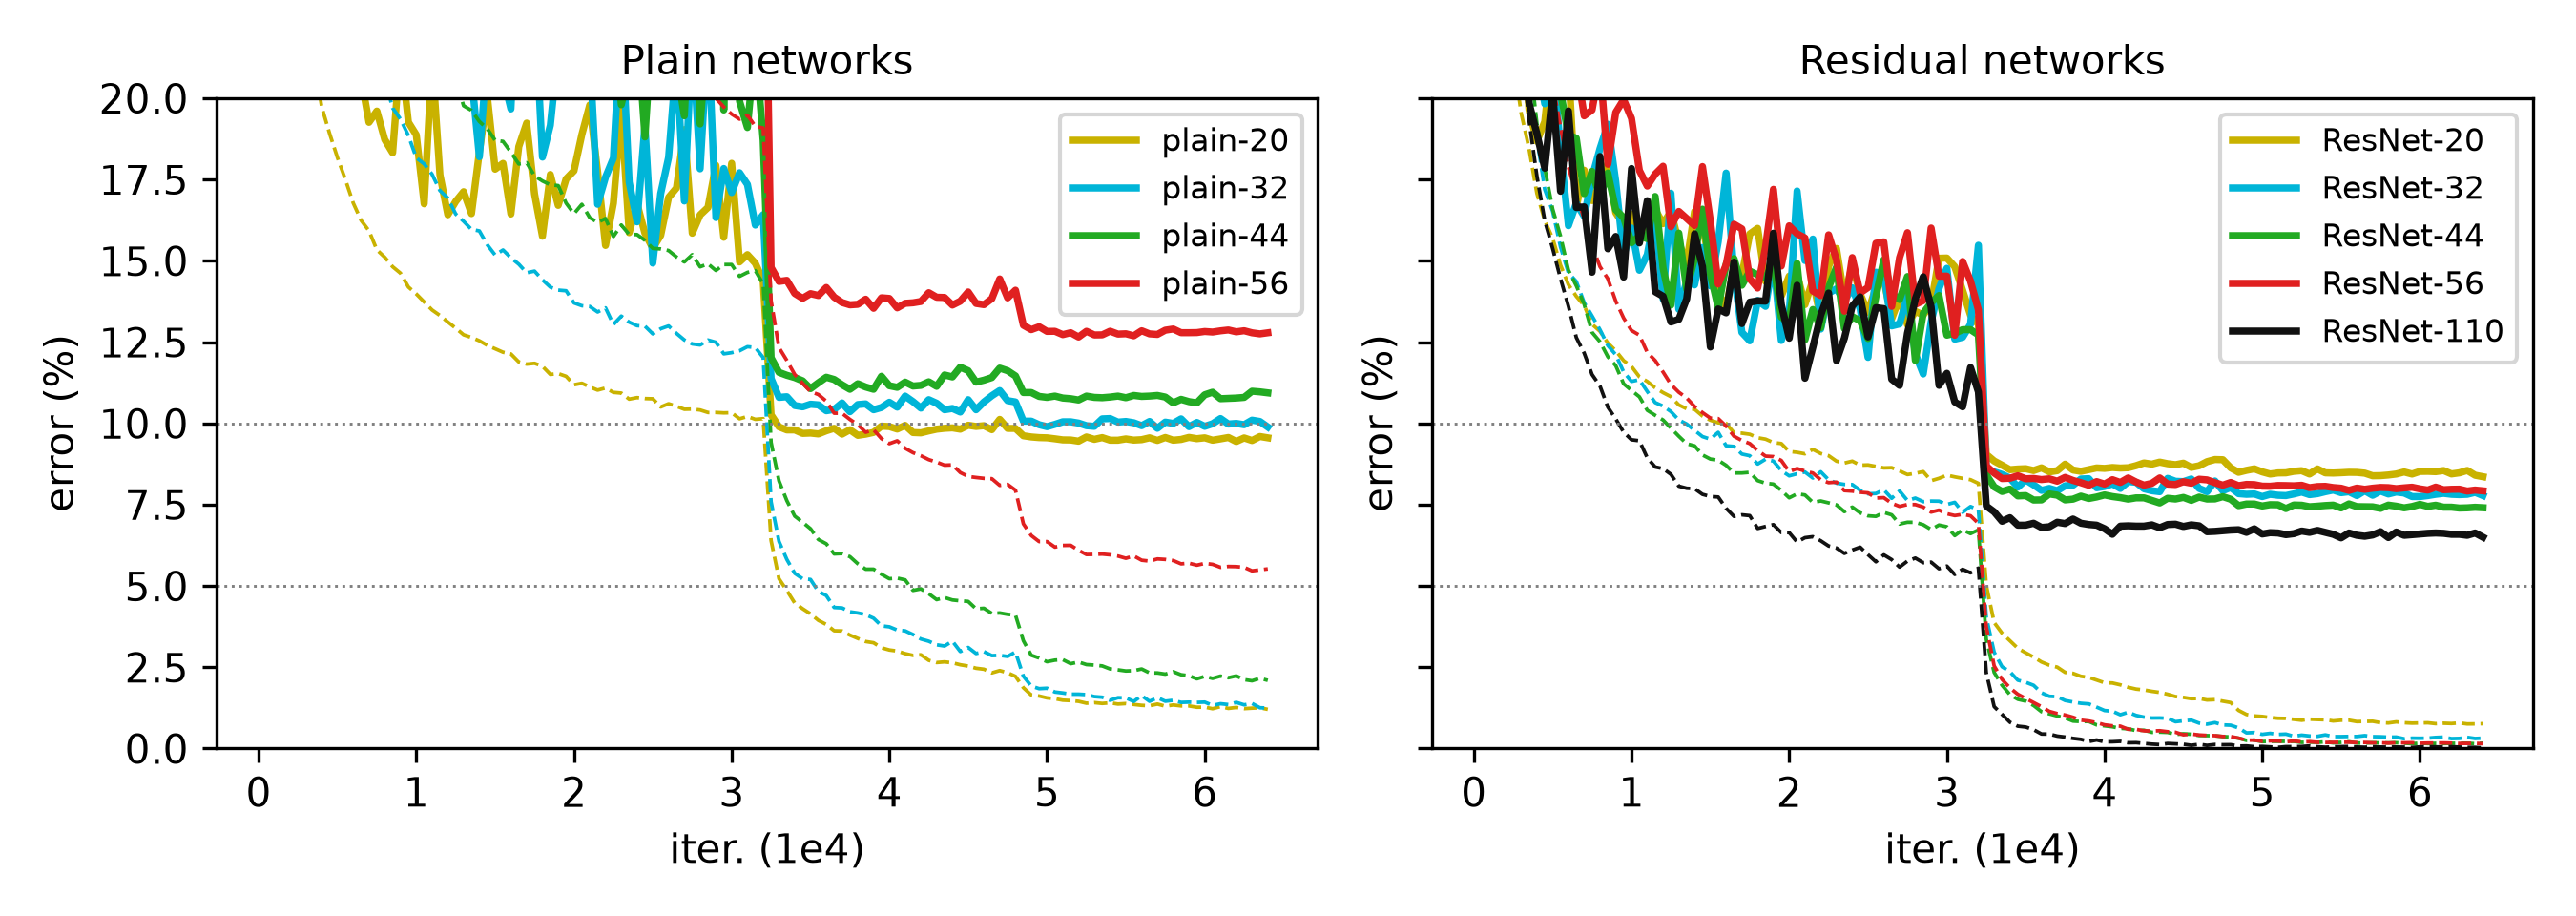
\includegraphics[width=0.85\textwidth]{fig6_side_by_side.png}
\caption{Training on CIFAR-10, reproducing Fig.~6 of \cite{he2016deep}. Dashed: training error (minibatches with augmentation). Bold: test error. Curves are averaged over the available seeds. Left: plain networks. Right: ResNets.}
\label{fig:curves}
\end{figure*}

\textbf{Plain networks degrade.} Test error rises with every increase in depth: \err{plain}{20}, \errmean{plain}{32}, \errmean{plain}{44} and \err{plain}{56}\%. The difference between 20 and 56 layers is far larger than the seed-to-seed spread. As in the paper, the deeper plain networks also have higher \emph{training} error throughout (Fig.~\ref{fig:curves}, left; final training error \trainerr{plain}{20}\% at 20 layers against \trainerr{plain}{56}\% at 56 layers), so the effect is not overfitting. The test-error gap between plain-56 and plain-20 is \cmpdiff{plain56-vs-20} points (Welch's $t=\cmpt{plain56-vs-20}$).

\textbf{Residual networks benefit from depth.} ResNet test error falls from \err{resnet}{20}\% at 20 layers to \errmean{resnet}{110}\% at 110 layers. ResNet-110 is within the paper's own spread ($6.61\pm0.16$\%), and ResNet-20 is \gap{20} points better than the paper's value. At every depth the residual network beats the plain network with the same parameters.

\textbf{Layer responses.} Fig.~\ref{fig:fig7} reproduces Fig.~7 of the paper. The mean standard deviation of 3$\times$3 layer responses is lower for ResNets than for plain networks of the same depth (\lstd{resnet}{56} against \lstd{plain}{56} at 56 layers) and falls with ResNet depth (\lstd{resnet}{20} at 20 layers to \lstd{resnet}{110} at 110), matching the paper's observation that deeper residual layers modify the signal less. One detail does not match: my plain networks' mean response also falls with depth, which the paper's figure does not show clearly.

\begin{figure}[t]
\centering
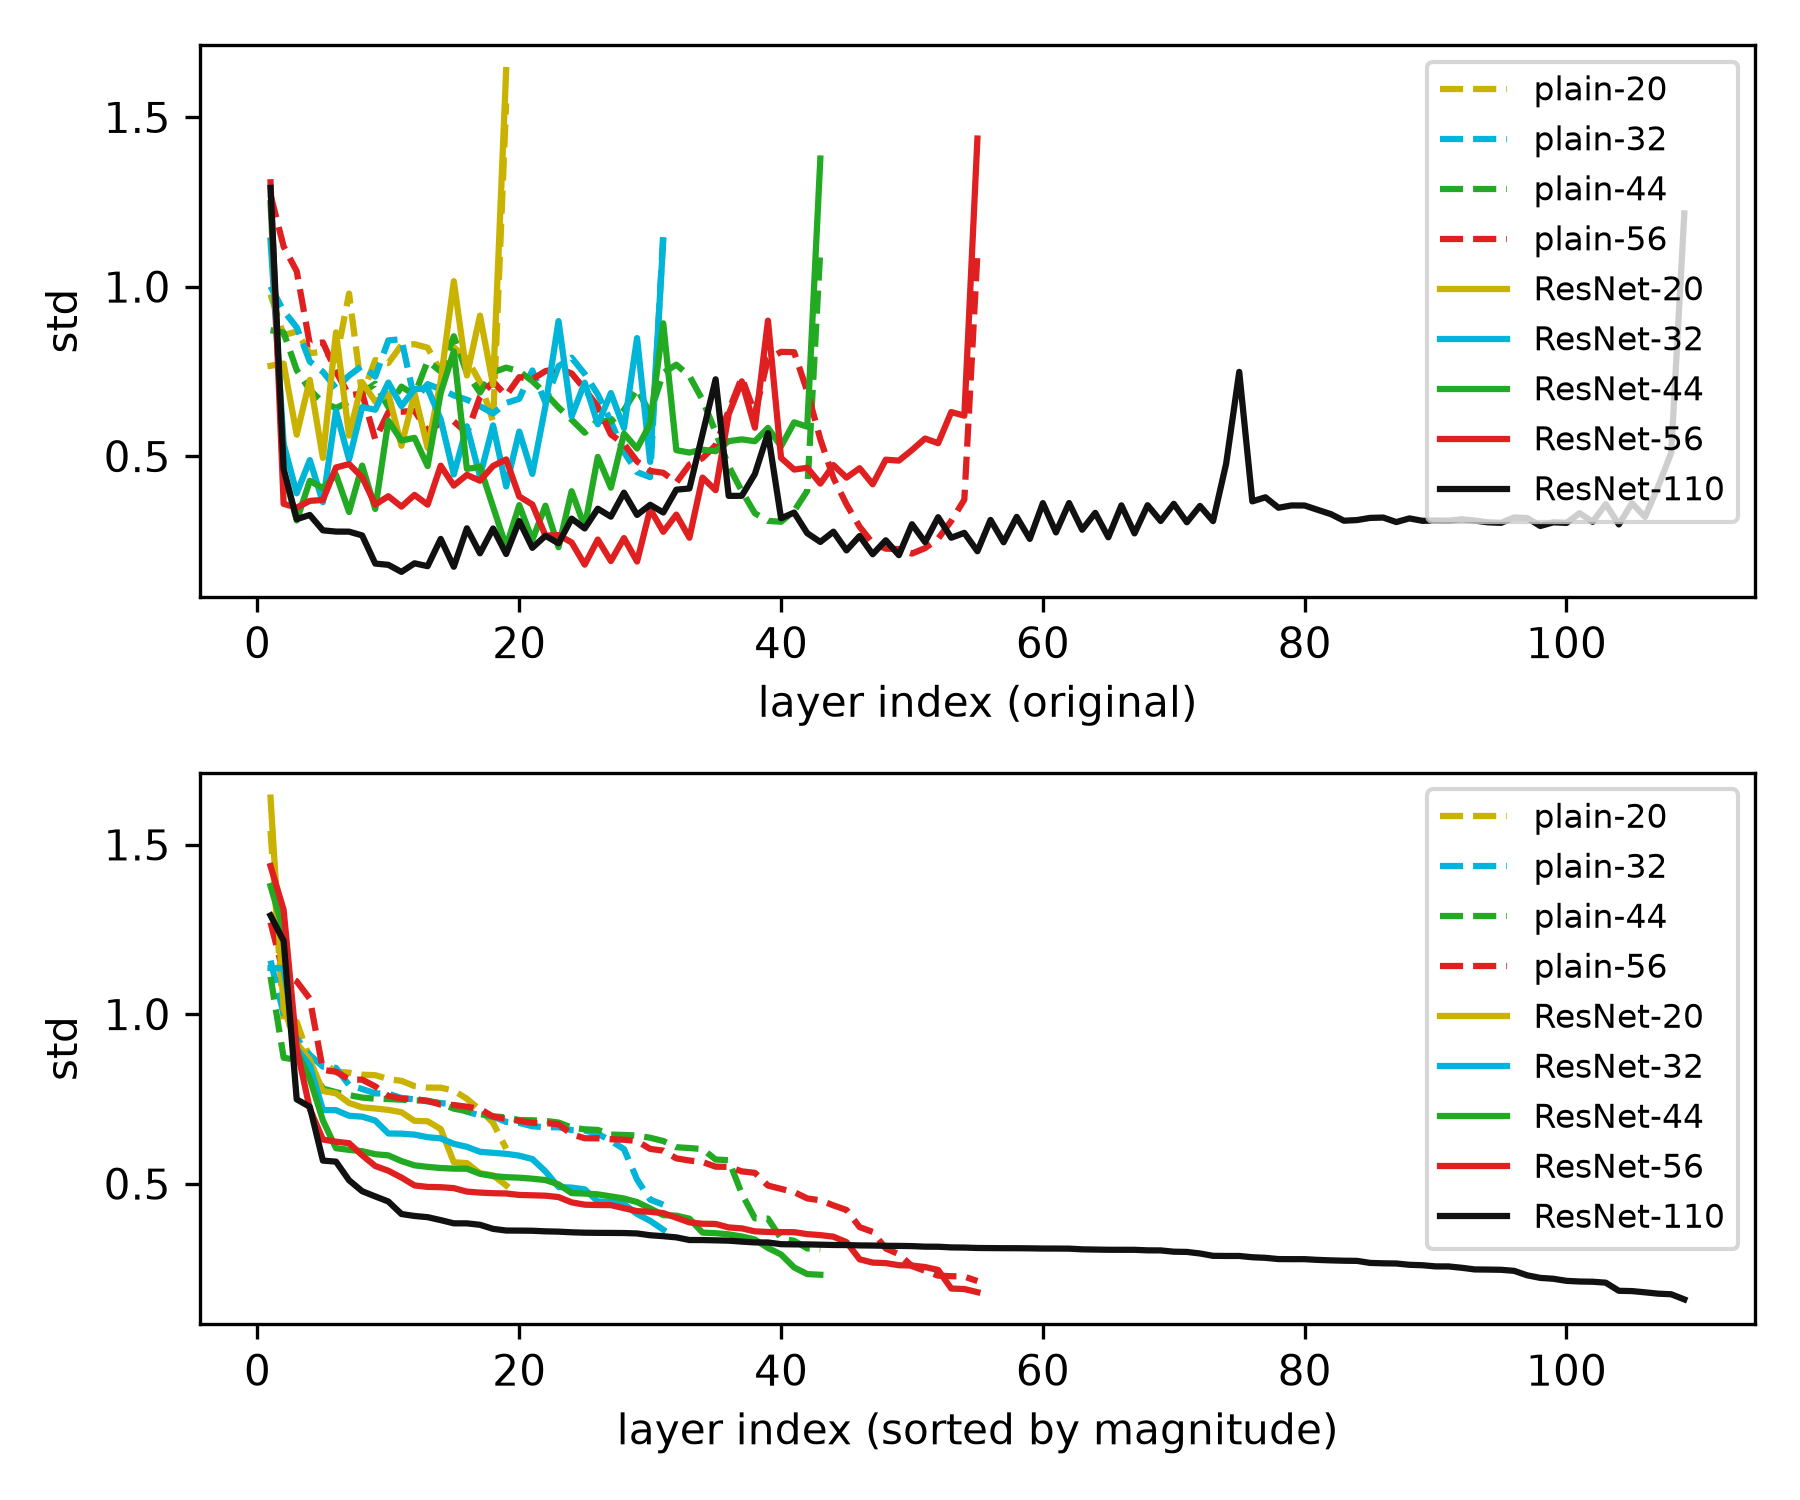
\includegraphics[width=\linewidth]{fig7_layer_std.png}
\caption{Standard deviation of each 3$\times$3 layer's response (after BN, before ReLU or addition) on the test set, seed 0. Top: original order. Bottom: sorted. Reproduces Fig.~7 of \cite{he2016deep}.}
\label{fig:fig7}
\end{figure}

\section{Numbers the Paper Does Not Report}
\label{sec:own}
\textbf{Seed variability.} The paper reports one run per model except ResNet-110. Over three seeds, plain-20 gives \err{plain}{20}\% and ResNet-56 \err{resnet}{56}\% (Tables~\ref{tab:main} and~\ref{tab:var}): seed-to-seed standard deviations of a few tenths of a point. This sets the scale against which any single-run difference in Table~6, such as the 0.20-point gap between ResNet-44 and ResNet-56, should be judged.

\textbf{Tabulated plain-network errors} for 20 to 56 layers (Table~\ref{tab:main}); the paper shows these only as curves.

\textbf{Projection shortcuts on CIFAR-10.} The paper compares option A and option B shortcuts only on ImageNet (its Table~3). ResNet-56 with option B scores \err{resnet}{56-B}\% over three seeds, against \err{resnet}{56}\% with option A: \cmpdiff{A-vs-B-56} points better (Welch's $t=\cmpt{A-vs-B-56}$), and within one standard deviation of the paper's option A value of 6.97\%. Option B adds only about 0.01M parameters (three 1$\times$1 convolutions), so the improvement is not explained by capacity. On ImageNet the paper found B only 0.5 points better than A for ResNet-34; on CIFAR-10 at 56 layers the difference in my runs is larger.

\textbf{Precision.} ResNet-56 trained in full FP32 scores \errmean{resnet}{56-fp32}\% (one run), indistinguishable from the FP16 runs (\err{resnet}{56}\%). Mixed precision therefore does not explain the gap; a single FP32 run cannot rule out a small effect, but any effect is smaller than the seed spread.

\begin{table}[t]
\caption{ResNet-44 and ResNet-56 runs used to investigate the gap (test error, \%)}
\label{tab:var}
\centering
\footnotesize
\resizebox{\linewidth}{!}{\begin{tabular}{@{}lccc@{}}
\toprule
Model and setting & Seeds & Each seed & Mean $\pm$ std \\
\midrule
ResNet-44, option A, FP16 (main) & 3 & 7.53, 7.06, 7.63 & 7.41 $\pm$ 0.30 \\
ResNet-56, option A, FP16 (main) & 3 & 8.04, 8.08, 7.66 & 7.93 $\pm$ 0.23 \\
ResNet-56, option B, FP16 & 3 & 6.83, 7.44, 6.92 & 7.06 $\pm$ 0.33 \\
ResNet-56, option A, FP32 & 1 & 7.95 & 7.95$^{\dagger}$ \\
\bottomrule
\end{tabular}
}
\end{table}

\section{The Gap}
\label{sec:gap}
\subsection{What did not reproduce}
Two results do not match the paper.

\emph{ResNet-56 is \gap{56} points worse than reported} (\err{resnet}{56}\% against 6.97\%). Even my best of three seeds, \errbest{resnet}{56}\%, is short of it. ResNet-32 and ResNet-44 are also behind, by \gap{32} and \gap{44} points, whereas ResNet-20 and ResNet-110 match or beat the paper. The shortfall is therefore concentrated in the middle depths.

\emph{ResNet-56 does not beat ResNet-44.} The paper's errors fall at every step in depth. In my runs, ResNet-44 (\err{resnet}{44}\%) is better than ResNet-56 (\err{resnet}{56}\%) by \cmpdiff{56-vs-44} points over three seeds each (Welch's $t=\cmpt{56-vs-44}$). The difference is larger than either model's seed spread, though with only three seeds per model it is suggestive rather than conclusive. The overall trend from 20 to 110 layers still holds, but the claim that \emph{each} additional block of depth helps does not reproduce at this step.

Neither failure is an optimisation failure. ResNet-56 ends with near-zero training error (\trainerr{resnet}{56}\%), so it fits the training data; the gap is in how well it generalises.

\subsection{What I tried}
\begin{enumerate}
\item \emph{More seeds.} Three seeds each for ResNet-44 and ResNet-56 test whether the ordering is noise. The ordering holds in the mean (ResNet-44 better by \cmpdiff{56-vs-44} points, larger than either seed spread), and the gap to the paper persists in every ResNet-56 seed (best \errbest{resnet}{56}\%).
\item \emph{Full precision.} Mixed precision is the largest numerical change from the paper. One FP32 run (\errmean{resnet}{56-fp32}\%) matches the FP16 mean, so precision is ruled out as the main cause.
\item \emph{Projection shortcuts.} Option B gives the channels that option A zero-pads a learned path at the three points where the shape changes. This closes the gap: \err{resnet}{56-B}\% over three seeds against the paper's 6.97\%.
\item \emph{Checking the implementation.} Parameter counts match Table~6 exactly; the learning-rate schedule, augmentation and test protocol were checked against the paper line by line; and ResNet-20 and ResNet-110 matching the paper argues against a gross error in the architecture or training loop.
\end{enumerate}

\subsection{What I still cannot explain}
The option B result locates the gap at the dimension-changing shortcuts, but not its cause. My option A follows the paper's description: subsample the input by taking every second pixel, then append zero channels. The paper does not specify how the subsampling is done (taking every second pixel or average pooling) or how the zero channels are placed, and either could matter at the three points where half the shortcut's channels carry no signal. I did not have time to test these variants. Other unstated details could also contribute:
\begin{itemize}
\item \emph{Reporting rule.} Table~6 gives the \emph{best} of five runs for ResNet-110. If other entries are also best-of-$k$, my means are not like for like; my best seeds narrow but do not close the gap.
\item \emph{Batch-normalisation details.} Caffe and PyTorch update the running statistics with different default averaging constants, and the paper does not say whether weight decay applies to batch-normalisation parameters. I apply it to all parameters.
\item \emph{Padding order.} I subtract the mean before zero-padding, so padded pixels equal the mean colour. Padding raw images first would pad with a different value. The paper does not specify the order.
\item \emph{Multi-GPU batch normalisation.} With two GPUs, the paper's batch statistics were probably computed over 64 images per GPU rather than 128.
\end{itemize}
I still cannot explain why the shortfall affects 32 to 56 layers but not 20 or 110 layers with the same option A shortcuts. ResNet-110 used the warm-up schedule and ResNet-20 is shallow enough to be insensitive, but these are guesses; ResNet-32 and ResNet-110 also have only one seed each, so their agreement or disagreement with the paper is less certain than the 3-seed results.

\subsection{Incidents}
One run (plain-56, seed 1) was interrupted by a power loss that corrupted its log file. It was deleted and retrained from the start, so every reported run completed all 64k iterations without interruption.

\section{Data Ethics}
\label{sec:ethics}
CIFAR-10 \cite{krizhevsky2009learning} contains 60,000 32$\times$32 images in ten object classes and has no person class, but people may appear incidentally in images. Its images were drawn from the 80 Million Tiny Images collection \cite{torralba2008tiny}, which was gathered automatically from web searches without the consent of the photographers or of anyone pictured. That parent collection was withdrawn by its creators in 2020 after an audit found offensive labels and non-consensual images \cite{prabhu2021large}. CIFAR-10's images were selected and relabelled by hand and the dataset remains available, but its distribution page states no formal licence. I used it only for research, did not redistribute it (the code downloads it from the official source), and the results here do not depend on any individual image.

\section{Conclusion}
The central claim reproduces: on CIFAR-10, deeper plain networks degrade, and identity shortcuts with no extra parameters reverse this, with ResNet-110 matching the paper. The finer-grained claim that ResNet error falls at every depth does not reproduce with zero-padding shortcuts: my option A ResNet-56 is \gap{56} points short of the paper and worse than ResNet-44 across three seeds. Changing only the three dimension-changing shortcuts to projections restores the paper's number, which points to an under-specified detail of option A rather than to the residual principle itself. Seed spreads of a few tenths of a point, which the paper does not report, also suggest that its single-run comparisons between neighbouring depths should be read with caution.

\bibliographystyle{IEEEtran}
\bibliography{refs}

\end{document}
